\documentclass[mathserif]{beamer}
%\usefonttheme{serif}
\usepackage[utf8]{inputenc}
\usepackage[T1]{fontenc}
\usepackage{lmodern}
\usepackage{etoolbox}
\usepackage{graphicx}
\usepackage{xcolor}
\usepackage{transparent}
\usepackage{hyperref}
\usepackage{amsmath}
\usepackage{tcolorbox}
\usepackage{parskip}
\usepackage[framemethod=tikz]{mdframed}
\usepackage{mathrsfs}
\usepackage{physics}
\usepackage{tikz, tikz-cd}
%\usepackage[citestyle=nature]{biblatex}
\usepackage{tensor}
\usepackage[absolute,overlay]{textpos}
\usepackage{tcolorbox}
\usepackage{bibentry}
\usepackage{bm}
\newcommand{\e}{\mathrm{e}}


\renewcommand\thefootnote{\textcolor{red!50!white}{\arabic{footnote}}}

\newcommand\FrameText[1]{%https://tex.stackexchange.com/a/32990/191229
	\begin{textblock*}{\paperwidth}(0pt,\textheight)
		\vspace{-2em}
		\raggedleft #1\hspace{2em}
\end{textblock*}}


\setbeamercolor{background canvas}{bg=black}
\usebackgroundtemplate{\tikz[overlay,remember picture] \node[opacity=1, at=(current page.center)] {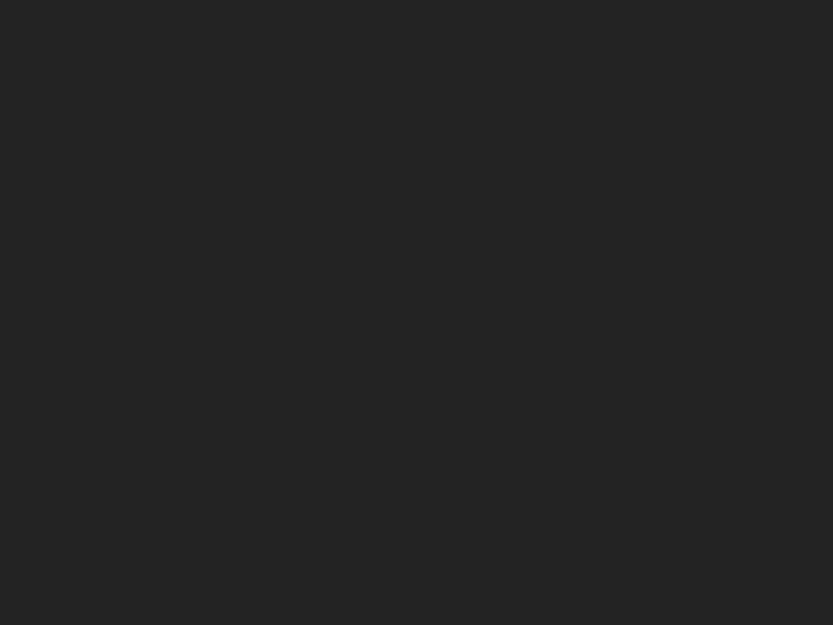
\includegraphics[height=\paperheight]{img/bakgrunn_plain.png}};
\FrameText{\href{https://www.twitter.com/Karlockert}{{\transparent{0.4}{\color{cyan!70!white}@karlockert}}}}
}


\setbeamertemplate{footline}[frame number]{}
% Fjerner navigasjonsbaren nederst
\setbeamertemplate{navigation symbols}{}
% Fjerner navigasjonssymbolene

%\addbibresource{bib.bib}

\begin{document}
	\color{white}
	%\usebackgroundtemplate{%             declare it
%	\tikz[overlay,remember picture] \node[opacity=1, at=(current page.center)] {
%		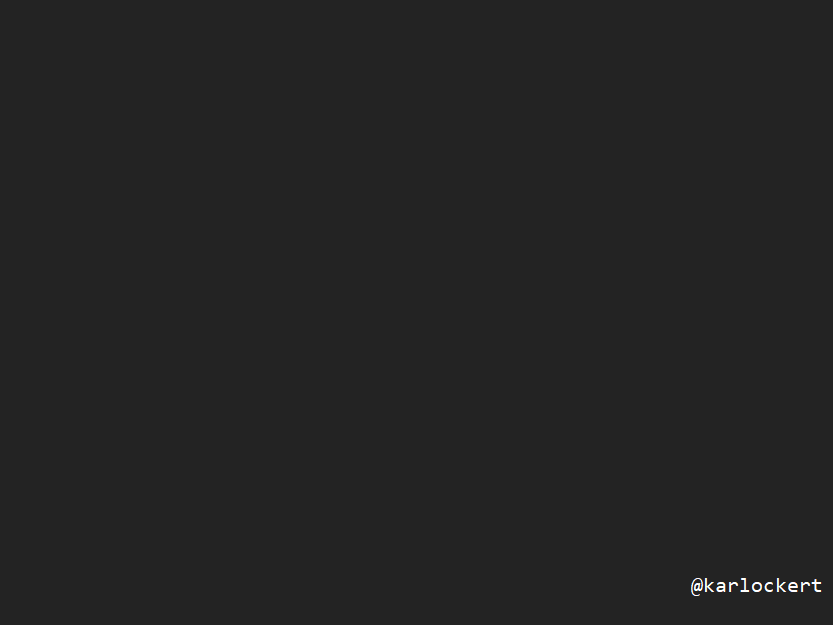
\includegraphics[height=\paperheight]{img/bakgrunn.png}};}

\begin{frame}[noframenumbering, plain]
	\begin{block}{\color{white}\textbf{\Large{
				%
					Title goes here
			%	
			}}}
		\vspace{-10pt}\rule{\textwidth}{0.5pt}
		\color{white}
		
		Some information about a cool theorem or anything i find interesting, related equations (here: Dirac-equation)
	
	\end{block}
	{\large
		
		\begin{equation*} 
			(i\gamma_{\mu}\partial^{\mu} - m)\psi = 0
		\end{equation*}
	}

	\begin{block}{}
	\color{white}
	
		Some more information here
		
	\end{block}
	

\end{frame}
	% Laget av: person

%\usebackgroundtemplate{%             declare it
%	\tikz[overlay,remember picture] \node[opacity=1, at=(current page.center)] {
%		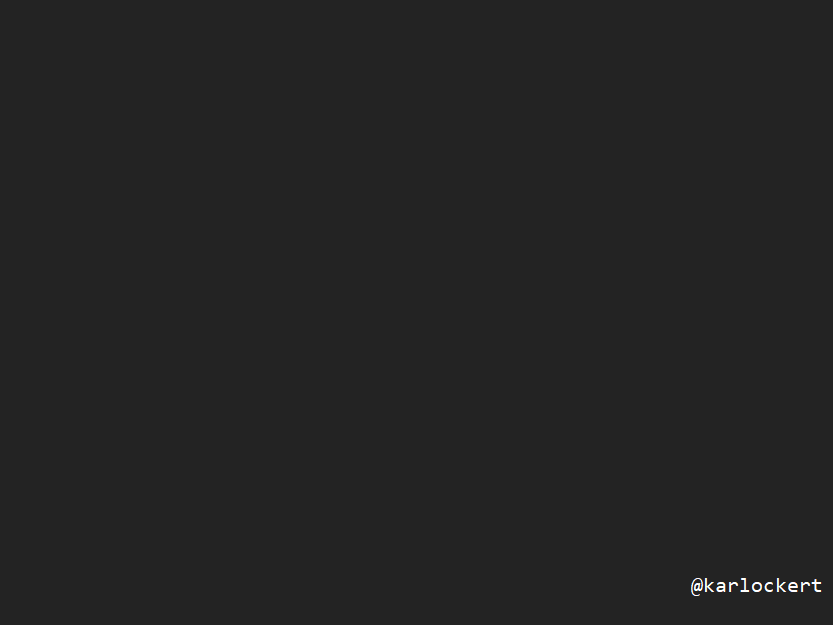
\includegraphics[height=\paperheight]{img/bakgrunn.png}};}
% Sett inn dit custom bilde her. template_background.png har riktig dimensjon, så om man vil redigere er det letteste å laste ned denne filen og redigere.

\begin{frame}[noframenumbering, plain]
	%	\frametitle{Hvis du ønsker}
	
	\begin{block}{\color{white}\textbf{\Large{Ehrenfests teorem }}}
		\vspace{-10pt}\rule{\textwidth}{0.5pt}
		\color{white}
		Hvorfor kollapser ikke bølgefunksjonen til hverdagslige ting (som f.eks. en stol)? Korrespondanseprinsippet forteller oss at i grensen av store antall partikler og høye energier, må kvantemekanikk være ekvivalent med klassisk fysikk. 
		Paul Ehrenfest fant en måte å relatere tidsutviklingen i forventningsverdien av kvantemekaniske operatorer til forventningsverdien av kraften som virker på systemet. Fra Newtons andre lov er dette forventet, men Ehrenfests teorem gir en matematisk trygghet. En generalisering av teoremet kan skrives på formen
	\end{block}
	{\large
		
		\begin{equation*} 
			\dv{t}\ev{O} = 	-i\hbar\ev{\comm{O}{\mathcal{H}}} + \ev{\pdv{O}{t}}	
		\end{equation*}
	}
	
	\begin{block}{}
		\color{white}
	hvor $O$ er en operator som korresponderer til en observerbar størrelse og $\mathcal{H}$ er Hamiltonian til systemet.
	\end{block}
\end{frame}
	%\usebackgroundtemplate{%             declare it
%	\tikz[overlay,remember picture] \node[opacity=1, at=(current page.center)] {
%		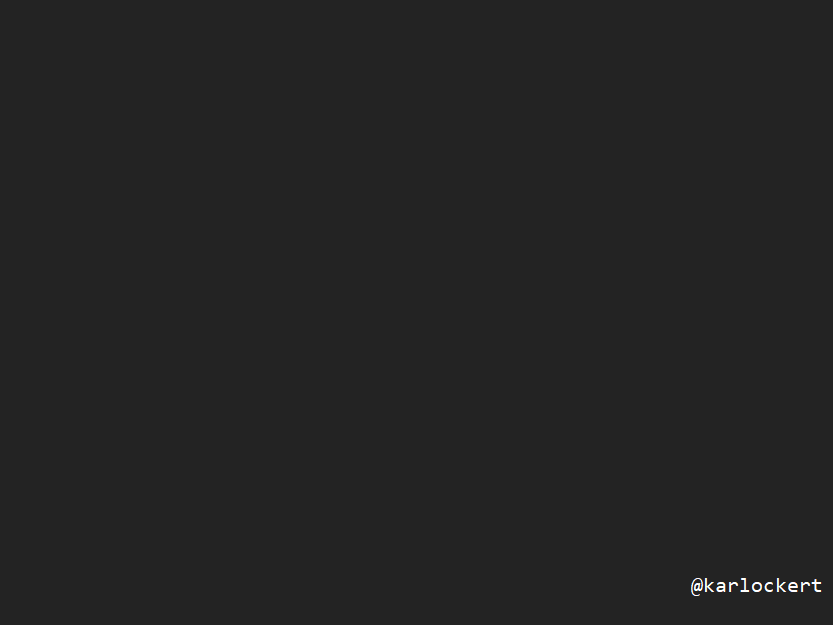
\includegraphics[height=\paperheight]{img/bakgrunn.png}};}

\begin{frame}[noframenumbering, plain]
%	\FrameText{@\href{https://www.twitter.com/Karlockert}{karlockert}}
	%	\frametitle{Hvis du ønsker}
	
		\begin{block}{\color{white}\textbf{\Large{The Hubbard Model }}}
			\vspace{-10pt}\rule{\textwidth}{0.5pt}
			\color{white}
			The Hubbard model is often called the ``Ising model'' of strongly correlated quantum systems, and an exact solution to this lattice model is only known in one dimension except in special limits.  
			It is given by the Hamiltonian 
		\end{block}
		{\large
			
%			\begin{tcolorbox}
				\begin{equation*}
					\mathcal{H} = - \sum_{i,j,\sigma}t_{ij}c_{i\sigma}^{\dagger}c_{j\sigma} + \sum_{i,\sigma}U_i n_{i,\sigma}n_{i,-\sigma}.
				\end{equation*}
%			\end{tcolorbox}
		}
	\begin{block}{}\color{white}
	where the first term is a tight-binding approximation of the system near its Fermi-energy, and the second term describes the on-site energy cost of having doubly occupied lattice sites. 
\end{block}
	%	hvor $O$ er en operator som korresponderer til en observerbar størrelse og $\mathcal{H}$ er Hamiltonian til systemet.
\end{frame}
	\begin{frame}[noframenumbering, plain]
	%\frametitle{Hvis du ønsker}
	
	\begin{block}{\color{white}\textbf{\Large{Hubbard-Stratonovich-transformasjonen}}}
		\vspace{-10pt}\rule{\textwidth}{0.5pt}
		\color{white}
		HS-transformasjon, også kalt HS-``dekobling'' er en nyttig identitet dersom du har for mange vekselvirkende fermioner i systemet ditt og heller ønsker en teori av (forhåpentligvis frie) bosoner.
		
	\end{block}
	
	{\large
		\begin{equation*}
			\e^{-\frac{a}{2}\psi^2} = \frac{1}{\sqrt{2\pi a}} \int\limits_{-\infty}^\infty\dd{\varphi} \e^{-\left(\frac{\varphi^2}{2a} +i\varphi\psi\right)}
		\end{equation*}
	}
	
	En diskret versjon av HS-dekoblingen kan for eksempel brukes til å transformere den kvantemekaniske Hubbard-modellen i $d$ dimensjoner til en klassisk Ising-liknende\footnote{\color{white}Multi-spin-vekselvirkende, i motsetning til den klassiske Ising-spin, som kun tar med par-spin-vekselvirkninger} modell i $d+1$ dimensjoner!
	
%	\fullcite{HSdecoupling}
	%\printbibliography
	%\bibliography{bib}
\end{frame}
	
	\section{Superconductivity}
	%\usebackgroundtemplate{%             declare it
%	\tikz[overlay,remember picture] \node[opacity=1, at=(current page.center)] {
%		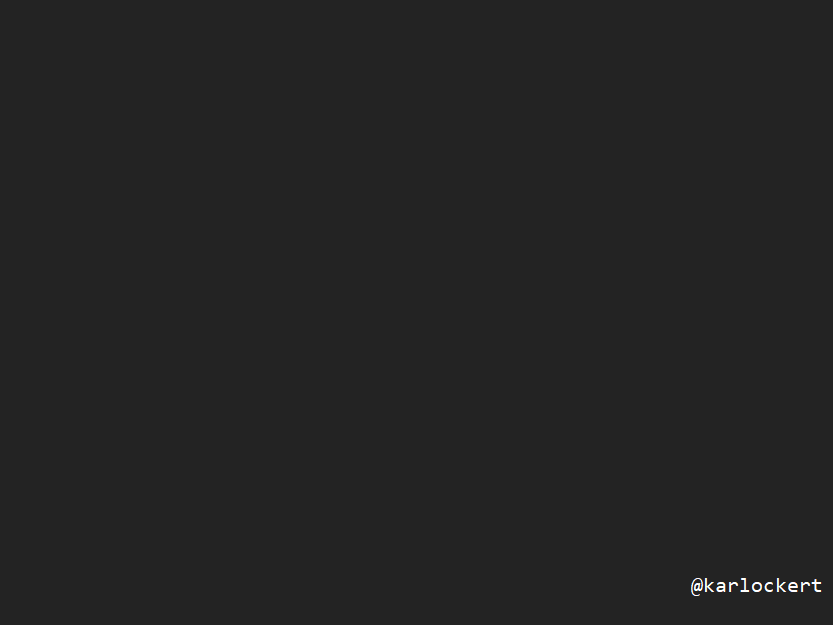
\includegraphics[height=\paperheight]{img/bakgrunn.png}};}

\begin{frame}[noframenumbering, plain]
	\begin{block}{\color{white}\textbf{\Large{
					%
					Superconductivity - BCS theory (1)
					%	
		}}}
		\vspace{-10pt}\rule{\textwidth}{0.5pt}
		\color{white}
		
	The Bardeen-Cooper-Schrieffer theory of superconductivity is the most celebrated microscopic theory describing the macroscopic phenomena of superconductivity. In this theory, an effective attractive potential between electrons in vicinity of the Fermi surface leads to the condensation of ``Cooper pairs'', reducing the free energy of the system. After some crude simplifications, a model Hamiltonian reads
		
	\end{block}
	{\large
		
		\begin{equation*} 
			\mathcal{H} = \sum_{k, \sigma}\varepsilon_kc_{k\sigma}^{\dagger}c_{k\sigma}  + \sum_{k, k'}V_{kk'}c_{k \uparrow}^{\dagger}c_{-k \downarrow}^{\dagger}c_{k'\downarrow}c_{k'\uparrow},
		\end{equation*}
	}
	
	\begin{block}{}
		\color{white}
		where $V_{kk'}$ is attractive in a thin shell close to the Fermi surface. This attractive potential can for instance be mediated by interacting with quantized lattice vibrations -- phonons. 
		
		
	\end{block}
	
	
\end{frame}




\begin{frame}[noframenumbering, plain]
	\begin{block}{\color{white}\textbf{\Large{
					%
					Superconductivity - BCS theory (2)
					%	
		}}}
		\vspace{-10pt}\rule{\textwidth}{0.5pt}
		\color{white}
		Since this Hamiltonian is quartic in fermion-operators, solving it exactly is very difficult. However, a mean field treatment is possible by letting $c_{-k\downarrow}c_{k\uparrow} = \ev*{c_{-k\downarrow}c_{k\uparrow}}$ + fluctuations, and the system might be solved. The self-consistent BCS gap-equation states
		
	\end{block}
	{
			\begin{align*}
					\Delta_k &= -\sum_{k'}V_{kk'}\Delta_{k'}\chi_{k'} \\
					\chi_{k} &= \frac{1}{\sqrt{\varepsilon_k^2 + \Delta_k^2}}\tanh(\frac{\beta}{2}\sqrt{\varepsilon_k^2 + \Delta_k^2}),
			\end{align*}

	}
	
	\begin{block}{}
		\color{white}
		where $\beta = \frac{1}{k_BT}$.
		This is a ``gap''-equation precisely because the condensation of Cooper pairs opens a gap $\Delta_k$ in the electronic excitation spectrum. A goal of modern physics is to find systems whose superconducting gap is as large as possible. 
		
		
	\end{block}
	
	
\end{frame}


\begin{frame}[noframenumbering, plain]
	\begin{block}{\color{white}\textbf{\Large{
					%
					Superconductivity - BCS theory (3)
					%	
		}}}
		\vspace{-10pt}\rule{\textwidth}{0.5pt}
		\color{white}
		
		The computation of $\Delta_k$ often requires heavy numerical computations, but some further analytic work can be done by assuming a constant attractive potential up to a Debye energy, where it is taken to be zero. 
		Remarkably, it turns out that the ratio of the gap $\Delta_k$ at zero temperature to the critical temperature (the temperature where $\Delta_k = 0$) is a purely numerical constant given by
		
	\end{block}
	{
		\begin{equation*} 
			\frac{\Delta(T=0)}{k_B T_C} = \pi\e^{-\gamma}, 
		\end{equation*}
	}
	
	\begin{block}{}
		\color{white}
		where $\gamma$ is the Euler-Mascheroni constant. This constant fits fairly well with the experimentally observed values for several materials, and reason to celebrate the BCS - theory as a whole. 
		
		
	\end{block}
	
	
\end{frame}
	%\usebackgroundtemplate{%             declare it
	%	\tikz[overlay,remember picture] \node[opacity=1, at=(current page.center)] {
		%		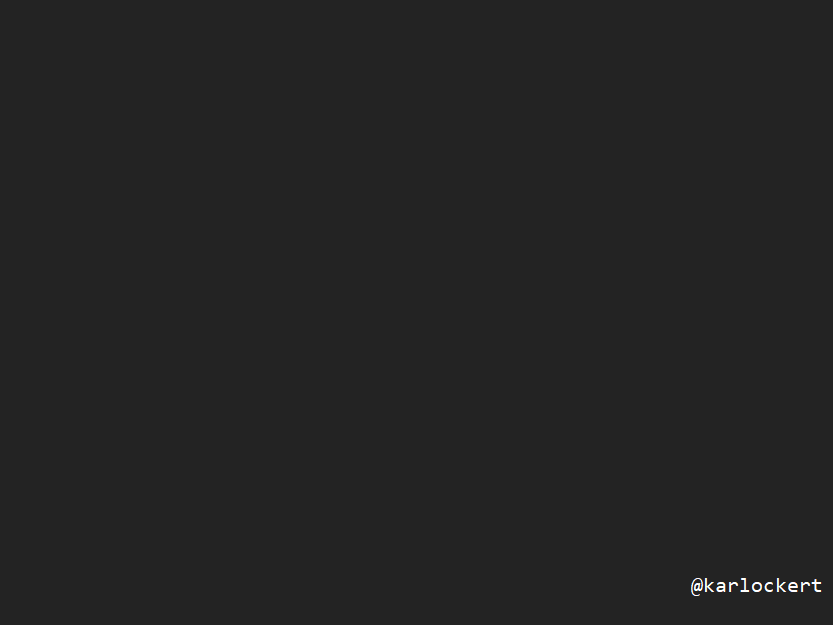
\includegraphics[height=\paperheight]{img/bakgrunn.png}};}

\begin{frame}[noframenumbering, plain]
	\begin{block}{\color{white}\textbf{\Large{
				Schrieffer-Wolff transformation
		}}}
		\vspace{-10pt}\rule{\textwidth}{0.5pt}
		\color{white}
		We have seen that attractive interactions between electrons give rise to a condensation of Cooper pairs and a finite gap in the electron band structure. 
		Kohn \& Luttinger proposed in 1965 a Cooper pairing mechanism with the assumption that the effective interactions between electrons is attractive. This mechanism is obtained by what is now called the Schrieffer-Wolff transformation, a unitary transformation of the interacting Hamiltonian
	\end{block}
	{\large
		\vspace{-2em}
		\begin{align*}
			\mathcal{H}' &= \e^{-S}\mathcal{H}\e^{S} \\
			&= \mathcal{H}_0 + V + \comm{\mathcal{H}}{S} + \frac{1}{2}\comm{\comm{\mathcal{H}}{S}}{S} +\dots
		\end{align*}
	}
	
	\begin{block}{}
		\color{white}
		\vspace{-3em}
		By choosing $S$ such that $\comm{\mathcal{H}_0}{S} = -V$, we obtain to $\order{V^2}$
\vspace{-1em}
		\begin{equation*}
				\mathcal{H}' = \mathcal{H}_0 + \frac{1}{2}\comm{V}{S} \equiv  \mathcal{H}_0 + V'
		\end{equation*}
Although this looks pretty similar to the starting point, this transformation is the first step of obtaining a gap equation for finite $T$, with unrestricted scattering momenta!	
\end{block}
	
	
\end{frame}
	
	\section{Topological Insulators}
	
	%\usebackgroundtemplate{%             declare it
	%	\tikz[overlay,remember picture] \node[opacity=1, at=(current page.center)] {
		%		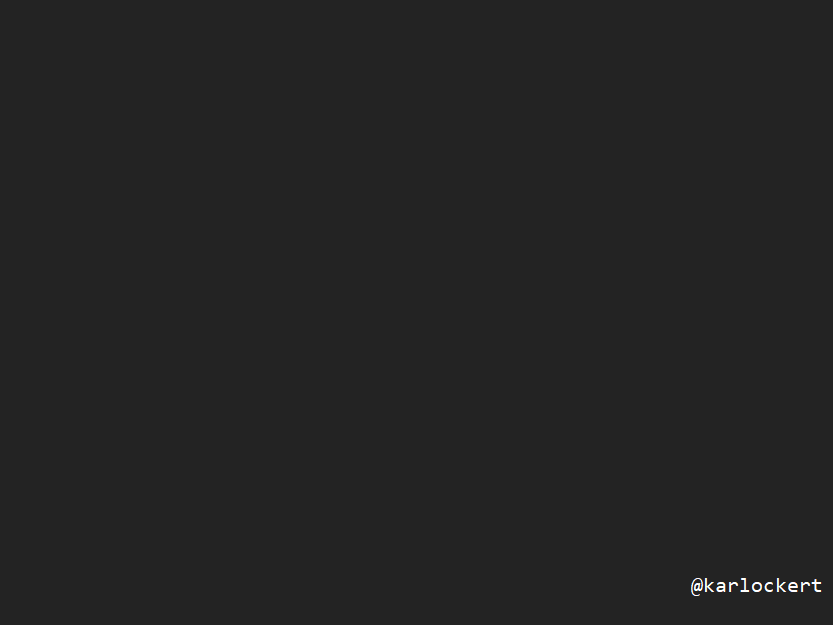
\includegraphics[height=\paperheight]{img/bakgrunn.png}};}

\begin{frame}[noframenumbering, plain]
	\begin{block}{\color{white}\textbf{\Large{
					%
					Topological Insulators - 1
					%	
		}}}
		\vspace{-10pt}\rule{\textwidth}{0.5pt}
		\color{white}
		
%		Topological insulators is a class of quantum matter with predicted properties relevant for the development of highly energy efficient information technologies such as spintronics.
		
		These materials are “topological” in the sense that certain quantities of the system is left invariant when it undergoes smooth transformations in the parameter space. An example of such a property is the Chern invariant $n$.
%		, which is associated with a quantized hall conductance. 
		
		This number can be calculated as the total Berry flux through the Brillouin zone from each band. 
		\begin{equation*}
			\label{eq:hamiltonian_pseudomagnetic}
			H(\bm{k}) = E_{\bm{k}}I + \vb d_{\bm{k}}\cdot\bm\sigma, 
		\end{equation*}
		the Chern number can be expressed in terms of the normalized vector $\hat{\vb{d}}_{\bm{k}} = \vb{d}_{\bm{k}} / |\vb{d}_{\bm{k}}|$ alone;
	
		
	\end{block}
	{\large
			\begin{equation*}
			n = \frac{1}{4\pi}\int_{1\text{BZ}}\dd[2]{\bm{k}}\hat{\vb{d}}_{\bm{k}} \cdot(\partial_{k_x}\hat{\vb{d}}_{\bm{k}}\cross\partial_{k_y}\hat{\vb{d}}_{\bm{k}}).
		\end{equation*}
	
	}
	
%	\begin{block}{}
%		\color{white}
%		
%		Some more information here
%		
%	\end{block}
\end{frame}


%\usebackgroundtemplate{%             declare it
	%	\tikz[overlay,remember picture] \node[opacity=1, at=(current page.center)] {
		%		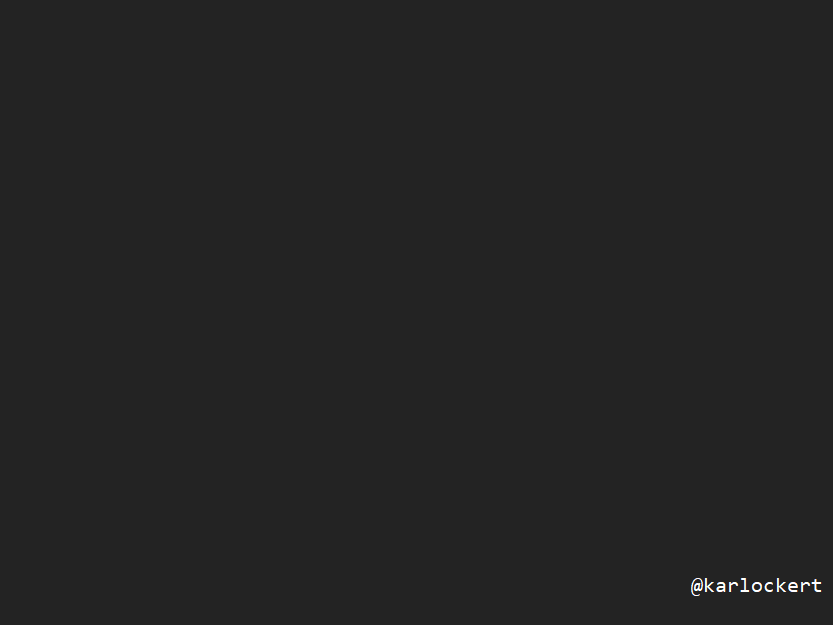
\includegraphics[height=\paperheight]{img/bakgrunn.png}};}

\begin{frame}[noframenumbering, plain]
	\begin{block}{\color{white}\textbf{\Large{
					%
					Topological Insulators - 2
					%	
		}}}
		\vspace{-10pt}\rule{\textwidth}{0.5pt}
		\color{white}
		
		%		Topological insulators is a class of quantum matter with predicted properties relevant for the development of highly energy efficient information technologies such as spintronics.
		
	
		Haldane showed in 1988 that for a particular model of the hexagonal lattice -- such as Graphene, the hall conductance is quantized in terms of this integer
	
		
	\end{block}
	{\large
		\begin{equation*}
		\sigma^{xy} = n\frac{2\pi e^2}{\hbar}
	\end{equation*}
		
	}
	
		\begin{block}{}
				\color{white}
				
				where the Chern number $n=0,\pm1$ is related to the number of edge states through what is now called the bulk-boundary correspondence. This model of spinless fermions on a hexagonal lattice is famously called the ``Haldane model''. The generalisation with spin degrees of freedom included led to the prediction of Spin Hall insulators -- a two dimensional rendition of a topological insulator.  
				
			\end{block}
\end{frame}

	
	\bibliography{bib.bib}

\end{document}

